\chapter{Dźwięk}
\label{cha:dwiek}

\section{Ogólna charakterystyka fal dźwiękowych}
Dźwięk jest wrażeniem słuchowym, powodowanym przez fale akustyczne. Rozchodzą się one w postaci fal podłużnych, będącymi zaburzeniami ciśnienia i gęstości ośrodka sprężystego\cite{FaleAkustyczne}. Prędkość dźwięku w powietrzu przy temperaturze 0 stopni celciusza wynosi 331,3m/s.

Dźwięk można opisać kilkoma podstawowymi parametrami:

\begin{itemize}
	\item wysokość (częstotliwość fali)
	\item głośność (amplituda fali)
	\item barwa (skład widmowy)
	\item czas trwania
\end{itemize}

Poziom dźwięku wyrażany jest miarą ciśnienia akustycznego, którego jednostką jest Paskal \textit{Pa}. Jednak ponieważ ludzkie ucho reaguje na bodźce logarytmicznie, częściej używa się decybeli ($\frac{1}{10}$ bela). Wzór na obliczenie poziomu ciśnienia akustycznego w skali logarytmicznej wygląda następująco\cite{CisnienieAkustyczne}:
\begin{equation}
SPL = 20\log{(\frac{p}{p_{ref}})}
\end{equation}

gdzie: \\
\indent$SPL$ - poziom ciśnienia akustycznego [\textit{dB}], \\
\indent$p$ - ciśnienie akustyczne [\textit{Pa}], \\
\indent$p_{ref}$ - ciśnienie akustyczne odniesienia, czyli próg słyszalności, wynoszący $2\cdot10^{-5} Pa$ 


\section{Odbiór fal dźwiękowych przez człowieka}
W ludzkim uchu odbiór dźwięku odbywa się przez zmiany ciśnienia płynu, którym wypełniony jest ślimak (patrz rys. \ref{slimak}). Powodują one podrażnianie rzęsek, które z kolei przekazują impulsy elektrochemiczne do mózgu. Im mniejsza częstotliwość fali, tym dalej ona dociera i na tej podstawie mózg potrafi rozróżniać częstotliwości. Dla człowieka słyszalne są fale z zakresu ok. 20Hz - 20kHz, choć górna granica maleje z wiekiem przez stopniową degradację najbardziej zewnętrznych rzęsek (a więc odpowiadających za najwyższe częstotliwości)\cite{JakSlyszymy}. 
Fale poniżej granicy słyszalności to infradźwięki, powyżej - ultradźwięki, a częstotliwości wyższe, niż $10^{10}kHz$ to hiperdźwięki.

\begin{figure}[H]
	\centering
	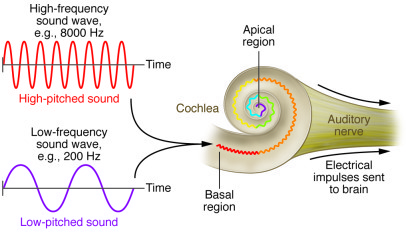
\includegraphics{zdjecia/slimak.png}
	\caption{\label{slimak} Odbiór fal dźwiękowych w ślimaku ludzkiego ucha\cite{cochlea}}
\end{figure}


\section{Fale dźwiękowe jako zagrożenie dla zdrowia człowieka}

Głównym, choć nie jedynym, parametrem dźwięku, który determinuje jego szkodliwość jest amplituda fali, czyli ciśnienie akustyczne. W tabeli \ref{tab:SPL} przedstawiono sytuacje, w których występuje określony poziom natężenia.

\begin{table}[H]
	\centering
	\begin{tabular}{|r|l|}
		\hline
		Natężenie [dB] & Sytuacja \\
		\hline
		\hline
		\rowcolor{red!50}
		130 & Młot pneumatyczny \\
		\hline
		\rowcolor{red!40}
		120 & Klakson z odległości 1m \\
		\hline
		\rowcolor{red!30}
		110 & Lotnisko \\
		\hline
		\rowcolor{red!20}
		100 & Przejazd pociągu \\
		\hline
		\rowcolor{orange!20}
		90 & Wnętrze autobusu \\
		\hline
		\rowcolor{yellow!20}
		80 & Zatłoczona ulica \\
		\hline
		\rowcolor{green!30}
		70 & Konwersacja \\
		\hline
		\rowcolor{green!30}
		60 & Salon z cichą muzyką \\
		\hline
		\rowcolor{green!30}
		50 & Biuro \\
		\hline
		\rowcolor{green!30}
		40 & Sypialnia \\
		\hline
		\rowcolor{green!30}
		30 & Studio nagraniowe \\
		\hline
		\rowcolor{green!30}
		20 & Studio radiowe \\
		\hline
	\end{tabular}
	\caption{Poziomy natężenia dźwięku\cite{SPLtable}}
	\label{tab:SPL}
\end{table}

Na szkodliwość dźwięku wpływa również czas jego trwania. Amerykańska agencja federalna NIOSH (ang. \textit{National Institute for Occupational Safety and Health}) zajmuje się badaniem i zapobieganiem chorobom związanym z pracą. Wydała ona dokument\cite{NIOSH}, w którym przedstawiono bezpieczny czas wystawienia na określone poziomy ciśnienia akustycznego\cite{SPLtable}.

\begin{table}[H]
	\centering
	\begin{tabular}{|r|l|}
		\hline
		Natężenie [dB] & Maks. czas [h] \\
		\hline
		\hline
		127 & 00:00:01 \\
		\hline
		118 & 00:00:14 \\
		\hline
		109 & 00:01:53 \\
		\hline
		100 & 00:15:00 \\
		\hline
		91 & 02:00:00 \\
		\hline
		82 & 16:00:00 \\
		\hline
	\end{tabular}
	\caption{Maksymalny czas wystawienia na określone poziomy natężęnia}
	\label{tab:SPLczas}
\end{table}

Odbiorcze uszkodzenie słuchu przez hałas nazywamy urazem akustycznym. Dzieli się go na ostry oraz przewlekły. Ostry jest powodowany krótkotrwałym oddziaływaniem natężenia powyżej 130dB, a przewlekły długotrwałym wystawieniem na dźwięki powyżej 85dB. W przypadku tego pierwszego uszkodzeniu ulega narzędzie Cortiego, będące częścią ślimaka i zawierające komórki rzęsate\cite{UrazyAkustyczne}.

\begin{figure}[H]
	\centering
	\begin{subfigure}{.45\textwidth}
		\centering
		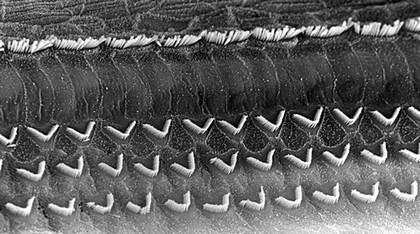
\includegraphics[scale=0.45]{zdjecia/cochlee-normale.jpg}
		\label{normal_cochlea}
		\caption{Zdrowe rzęski}
	\end{subfigure}
	\begin{subfigure}{.45\textwidth}
		\centering
		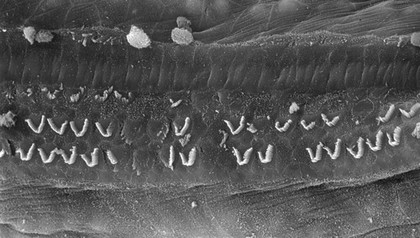
\includegraphics[scale=0.44]{zdjecia/traumatisme-sonore-niveau-2.jpg}
		\label{damaged_cochlea}
		\caption{Uszkodzone rzęski}
	\end{subfigure}
	\caption{Powierzchnia ślimaka widoczna pod mikroskopem elektronowym\cite{RzeskiMikorskop}}
\end{figure}


\subsection{Dźwięki strzałów i wybuchów}

W trakcie rozważań szczególną uwagę poświęcono dźwiękom pochodzącym od broni palnej. To właśnie one miały być głównym źródłem zagrożenia dla słuchu użytkownika. 
Ich źródłem jest eksplozja prochu strzelniczego, zmagazynowanego w łusce naboju, która nadaje prędkość początkową pociskowi. Ciśnienie akustyczne podczas takiego wybuchu przekracza $ 140 dB $, a więc wystarczy niecała sekunda, aby doprowadzić do uszkodzenia słuchu\ref{tab:SPLczas}. Dodatkowo na takie uszkodzenie najbardziej narażone są rzęski odpowiedzialne za częstotliwości między $ 3 $ a $ 6kHz $\cite{BadaniePolicjantow}. 

Aby sprawdzić częstotliwości wystrzałów różnych typów broni, zaimplementowany został program w \textit{Pythonie} do analizy dźwięków z plików \textit{.wav}. Miał on za zadanie odczytać przebieg sygnału z pliku, odfiltrować częstotliwości powyżej $ 15kHz $ i przeprowadzić szybką transformatę Fouriera na odfiltrowanym sygnale. Kod źródłowy dostępny jest na repozytorium pod linkiem \url{https://github.com/Hoplophile/Tactical_Headphones_Sim.git}. 

Schemat działania programu wygląda następująco:

\begin{figure}[H]
	\centering
	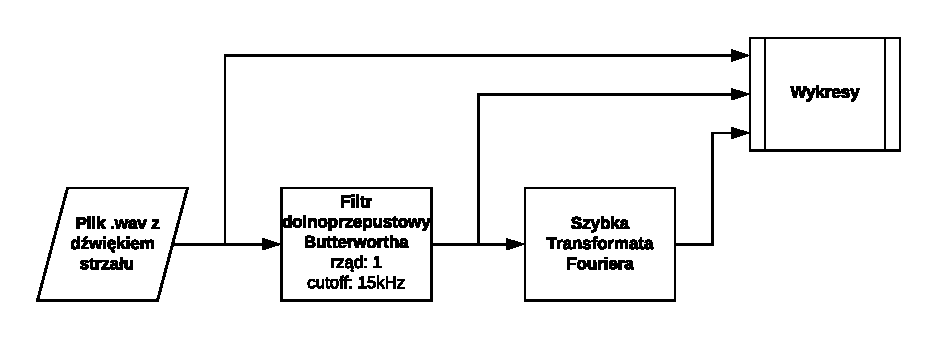
\includegraphics[scale=1]{grafy/Python_analiza_FFT.pdf}
	\caption{\label{graf:analizaFFT} Dataflow programu do analizy FFT}
\end{figure}

Pliki źródłowe z dźwiękami broni zostały pobrane ze strony \url{http://soundbible.com/tags-gun.html}. To powodowało brak pewności, czy dźwięk faktycznie pochodzi od broni podanej w nazwie oraz brak powtarzalności dźwięków, które nagrywane były w innych środowiskach, nieznanej odległości od broni i mikrofonami o różnych parametrach. Było to jednak najlepsze dostępne źródło tego typu nagrań. Wybrane zostały 4 pliki podpisane następującymi typami broni:

\begin{itemize}
	\item \textbf{M4A1} - karabin szturmowy kalibru 5.56mm
	\item \textbf{AK-47} - karabin szturmowy kalibru 7.62mm
	\item \textbf{Beretta M92} - pistolet kalibru 9mm
	\item \textbf{Mossberg 500} - strzelba (kaliber nieznany)
\end{itemize}

Program zwracał osobne wykresy dla każdego pliku źródłowego przedstawione poniżej.

\begin{figure}[H]
	\centering
	\begin{subfigure}{.49\textwidth}
		\centering
		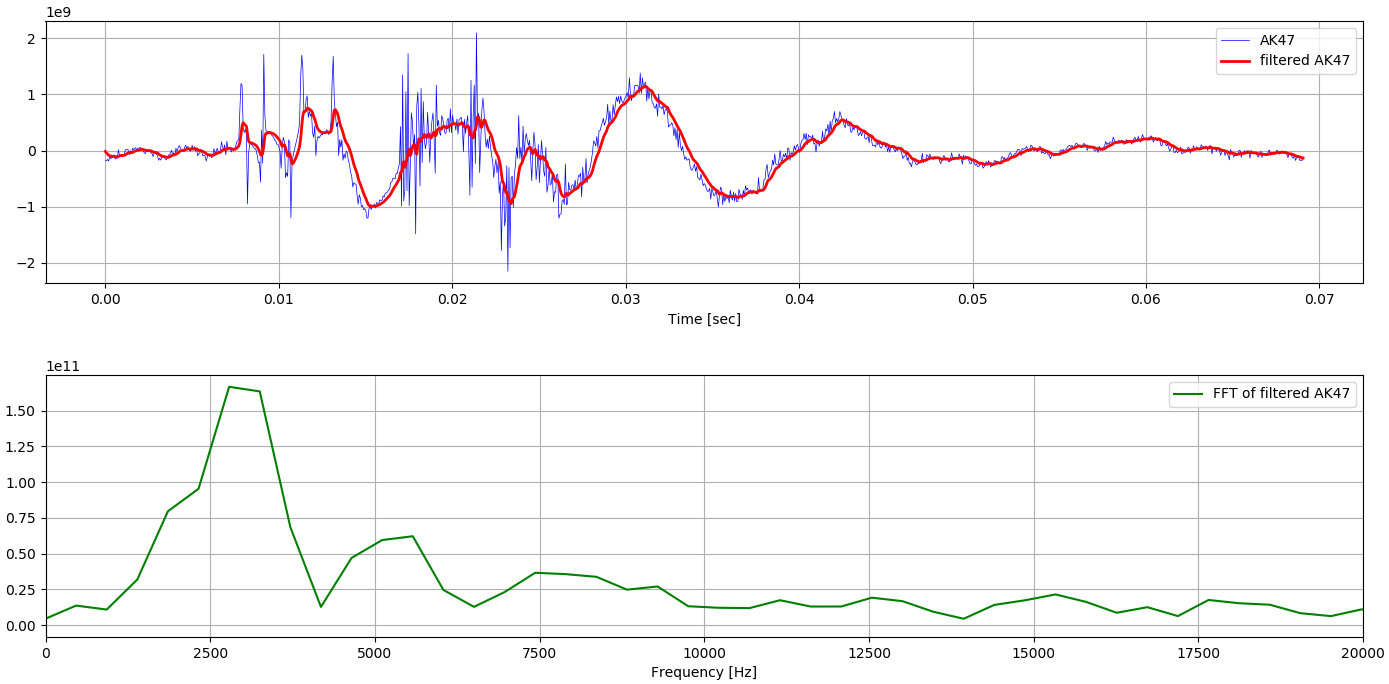
\includegraphics[height=3.9cm]{wykresy/AK47_fft.png}
		\subcaption{AK-47}
	\end{subfigure}
	\begin{subfigure}{.49\textwidth}
		\centering
		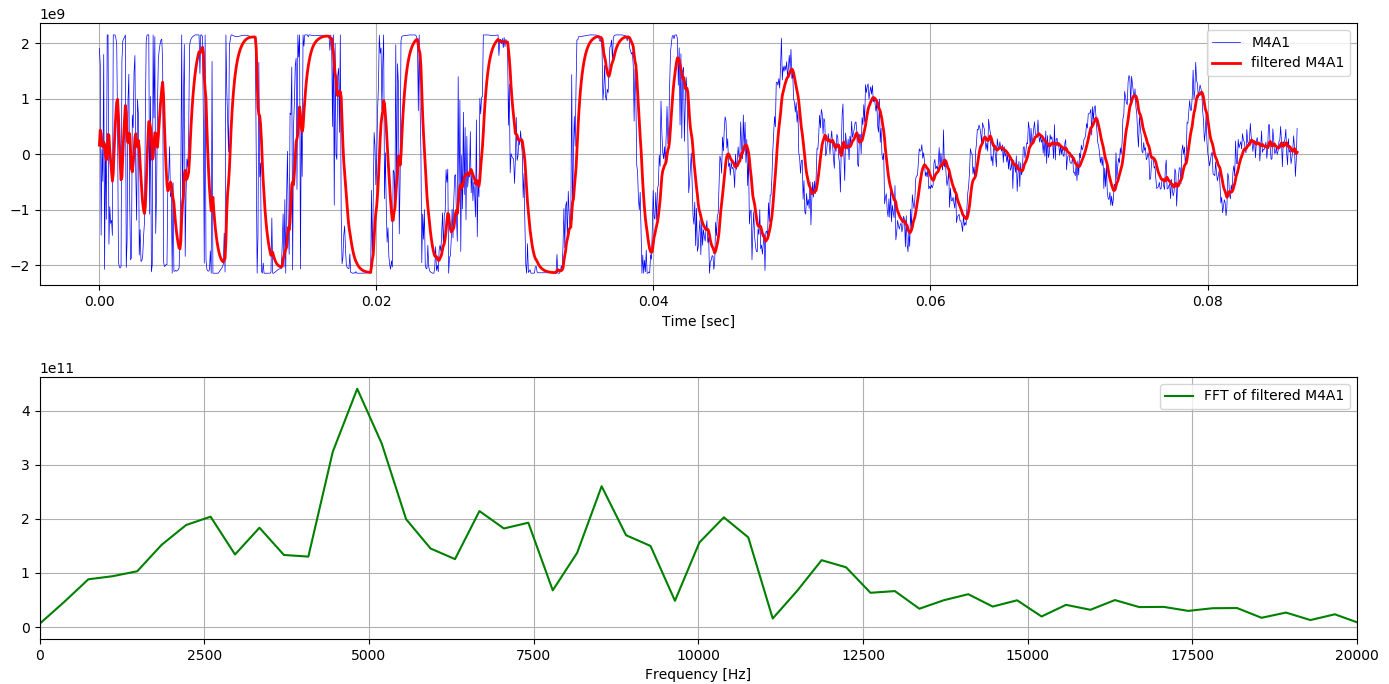
\includegraphics[height=3.9cm]{wykresy/M4A1_fft.png}
		\subcaption{M4A1}
	\end{subfigure}
	\begin{subfigure}{.49\textwidth}
		\centering
		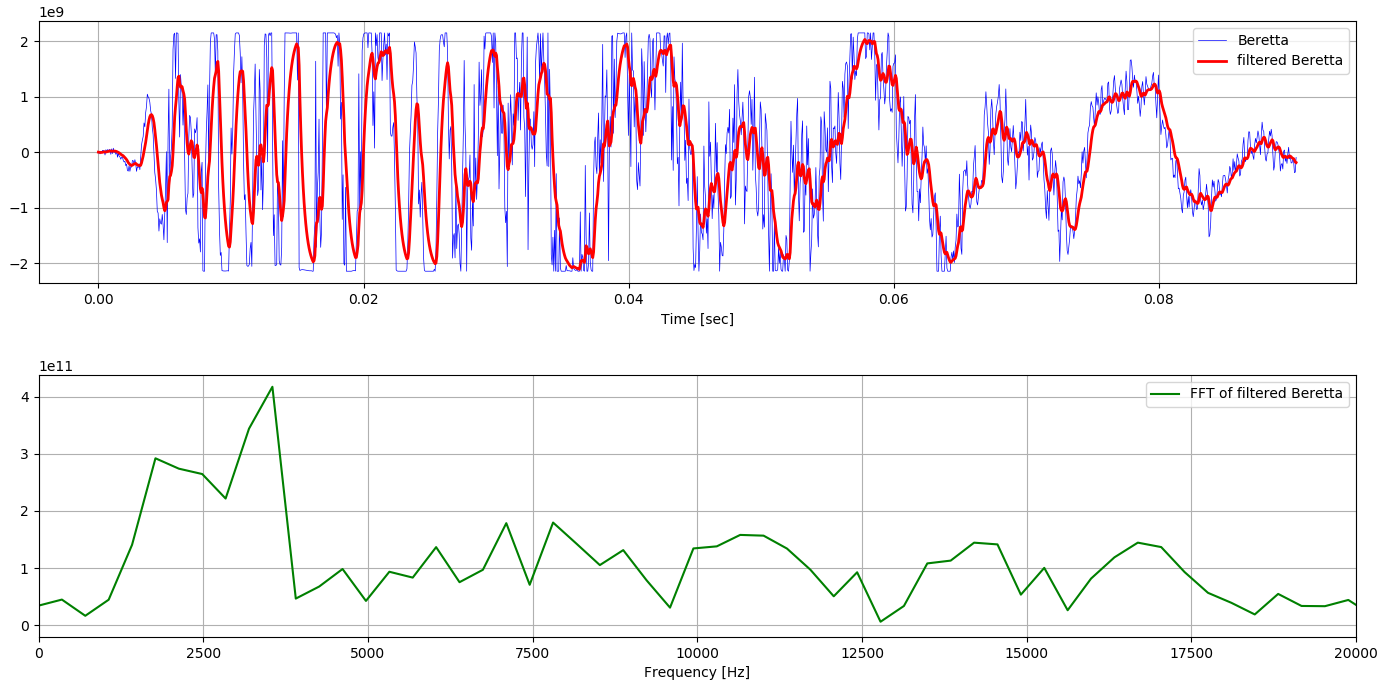
\includegraphics[height=3.9cm]{wykresy/Beretta_fft.png}
		\subcaption{Beretta M92}
	\end{subfigure}
	\begin{subfigure}{.49\textwidth}
		\centering
		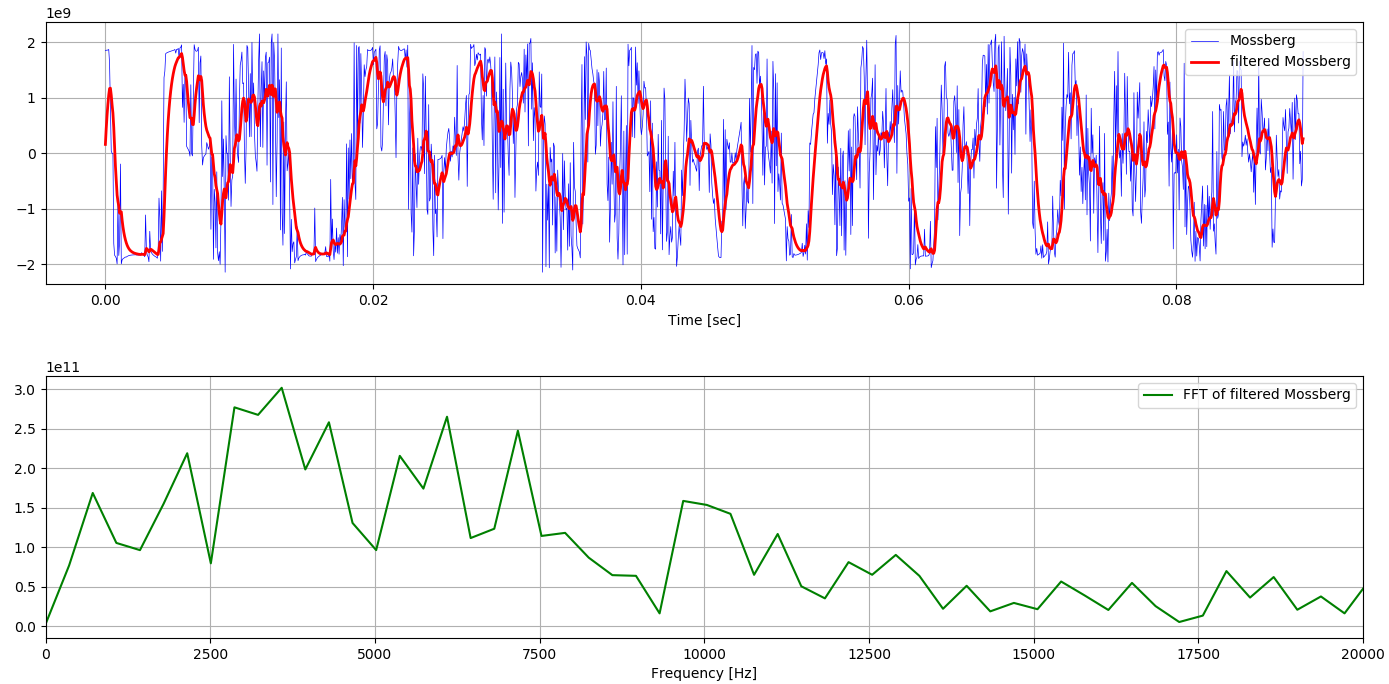
\includegraphics[height=3.9cm]{wykresy/Mossberg_fft.png}
		\subcaption{Mossberg 500}
	\end{subfigure}
	\caption{\label{pic:wykresy_FFt} Wykresy z analiz FFT dźwięków strzałów}
\end{figure}

Mimo, że nie udało się doprowadzić do przedstawienia większej liczby punktów na wykresie FFT, to z pewną dokładnością można stwierdzić, że dla wszystkich dźwięków największy pik mieści się w zakresie $ 3-6kHz $. Dodatkowo na wykresach przedstawiających oryginalny przebieg sygnału widać, że mikrofony w większości przypadków osiągnęły poziom nasycenia (wypłaszczenia na granicach osi y). To wpływa negatywnie na jakość transformaty i oznacza, że dźwięk osiągnął poziom nasycenia mikrofonu, która zwykle wynosi między $ 110 $ a $ 130 dB $. 

Powyższa analiza wskazuje na to, że zarówno częstotliwości, jak i natężenia dźwięków strzałów z broni palnej czyni je szczególnie niebezpiecznymi dla słuchu.
